\scanpage{20}\mspage{19}
de ce type si $L$ est fini). Donc on se bornera donc aux $\unsure{\mathscr{L}|\Phi}\in\unsure{\mathcal F|\mathscr F}$ telles que les $A\in\mathscr{L}$ soient fermés de $L$, i.e. telle que
\[ \mathscr{L}\subset\unsure{\mathcal P|\mathfrak P}_{\text{fermés}}(L) \]
Les \unsure{élément|éléments} de $\mathcal F'$ ainsi \unsure{obtenu|obtenus} peuvent s'interpréter en termes de $X$, comme des familles admissibles \inserted{(mais oui)} de familles de
parties \inserted{fermées} de $X$, \inserted{chacune} \uline{stables} par la relation d'équiv. des \deleted{cellules} \inserted{strates} ouvertes $X_{\unsure{\circ|a|\bullet|\cdot}}^\circ$, i.e. chacune réunion de strates fermées de $X$.
Dans une terminologie qui sera développée, elles \deleted{sont}\inserted{admettent} donc toutes le recouvrement donné de $X$ comme une ``subdivision''\unsure{;|,} (ou \unsure{plus tôt|plutôt}, \inserted{celui} induit sur leur support dans $X$)

\figure{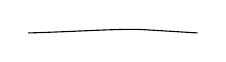
\begin{tikzpicture}\draw (0,0) .. controls (0.7,0.02) and (1.2,0.06) .. (1.5,0.04) -- (2.15,0);\end{tikzpicture}}

Soient $\deleted{\unsure{\Phi}}F$ et $G$ deux figures ensemblistes de $L$. On veut définir quand $F$ est un \uline{raffinement}, et quand c'est une \uline{subdivision} de $G$.

\uline{Proposition} Conditions équivalentes

% slanted
\margin{Cela implique $|\deleted{\unsure{A}}F|\subset|G|$}
a) $[$ $\forall\unsure{a|\cdot}\;A\in F$, désignant par $G\deleted{{}_A}{}^A$ l'ens des $B\in G$ tels que $A\subset B$, $G\deleted{{}_A}{}^A$ a un plus petit
élément $\varphi(A)$. (On trouve donc une application $\varphi:\deleted{\unsure{A}}F\longrightarrow G$, qui est bien sur croissante.) $]$ De plus
